\documentclass[unicode]{beamer}

\mode<presentation>
{
  \usetheme{Madrid}       % or try default, Darmstadt, Warsaw, ...
  \usecolortheme{default} % or try albatross, beaver, crane, ...
  \usefonttheme{default}    % or try default, structurebold, ...
  \setbeamertemplate{navigation symbols}{}
  \setbeamertemplate{caption}[numbered]
} 

\usepackage{cmap}
\usepackage[ukrainian]{babel}
\usepackage[utf8]{inputenc}
\usepackage[T2A]{fontenc}
\usepackage{chemfig}
\usepackage[version=3]{mhchem}
\usepackage{amsthm,amsmath,amssymb}
\usepackage{graphicx}

% On Overleaf, these lines give you sharper preview images.
% You might want to `comment them out before you export, though.
\usepackage{pgfpages}
\pgfpagesuselayout{resize to}[%
  physical paper width=8in, physical paper height=6in]

% Here's where the presentation starts, with the info for the title slide
\title[]{Розподілені алгоритми пошуку рівноваги Неша}
\author[Півень Д.М.]{Півень Денис Миколайович}
\institute[]{Науковий керівник:\\
професор, доктор фіз.-мат. наук\\
\normalsize{Семенов Володимир Вікторович}\\
\vspace{5mm}
\textsuperscript{Кафедра обчислювальної математики}
}
\date{14 червня 2022 р.}

\begin{document}

\begin{frame}
  \titlepage
\end{frame}

\begin{frame}{Теорія ігор}
    \begin{rows}
	\row{\textwidth}
    \begin{itemize}
        \item теорія математичних моделей прийняття оптимальних рішень в умовах конфлікту\\
        \item розділ прикладної математики, який використовується в економіці, біології, політичних науках, комп'ютерних науках
    \end{itemize}
\bigskip
	\row{\textwidth}
	\begin{figure}
		\centering
		% Requires \usepackage{graphicx}
		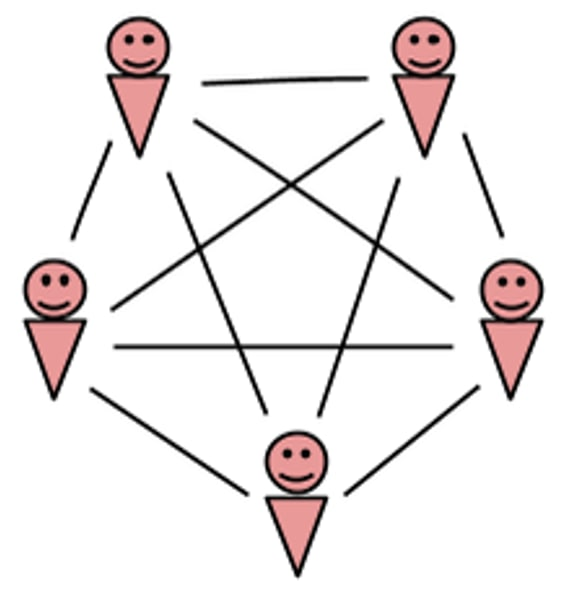
\includegraphics[width=5cm]{Game theory.jpg}
		\label{secert_sharing_figures}
	\end{figure}
\end{rows}
\end{frame}

\begin{frame}{Джон Форбс Неш}
\begin{columns}
	\column{0.5\textwidth}
\begin{itemize}
    \item американський математик, що зробив значний внесок у розвиток теорії ігор та диференціальної геометрії\\
    \item лауреат Нобелівської премії з економіки 1994 року\\
    \item лауреат Абелівської премії 2015 року
\end{itemize}
    \bigskip
	\bigskip
	\bigskip
	\bigskip
	\bigskip
	\bigskip
	\column{0.5\textwidth}
	\begin{figure}
		\centering
		% Requires \usepackage{graphicx}
		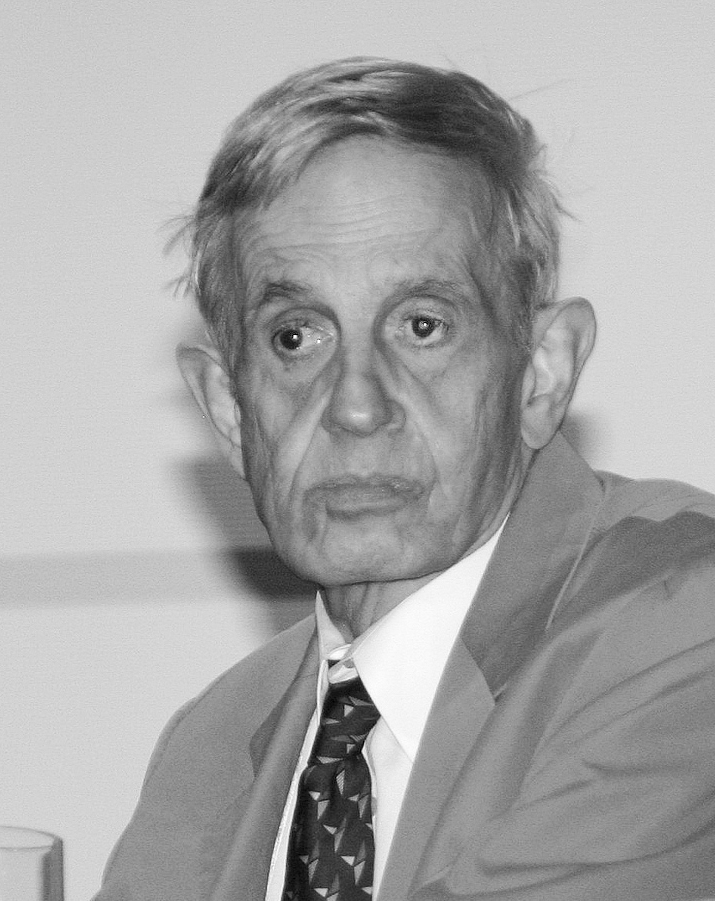
\includegraphics[width=5cm]{John Nash.jpg}
		\caption{Джон Форбс Неш}
		\label{secert_sharing_figures}
	\end{figure}
\end{columns}
\end{frame}

\begin{frame}{Рівновага Неша}
\begin{columns}
	\column{0.5\textwidth}
\begin{itemize}
    \item ситуація, при якій жоден з учасників не може збільшити свій виграш, змінивши вибір стратегії в односторонньому порядку, коли інші учасники не змінюють свого вибору.
\end{itemize}
    \bigskip
	\column{0.5\textwidth}
	\centering
	\begin{tabular}{ | c | c | c | }
\hline
 & A & B \\ \hline
A & 1; 1 & 10; 0 \\
\hline
B & 0; 10 & *2; 2^\bullet \\
\hline
\end{tabular}
\end{columns}
\end{frame}

\begin{frame}{Розподілені ігри}
\begin{itemize}

\item Агрегативна гра --- це гра, в якiй виграш кожного гравця є функцiєю власної стратегiї гравця та сукупностi стратегiй усiх гравцiв.

\item У нашому випадку гра є мережевою, тобто кожен гравець спiлкується з iншими гравцями та отримує iнформацiю про їхнi стратегiї.

\item Гра вiдбувається покроково, спочатку всi гравцi обирають випадкову стратегiю, далi вони повiдомляють її своїм «знайомим» та отримують iнформацiю про їхнi стратегiї, змiнюють свою стратегiю деяким чином, далi процес продовжується доки кожному гравцю буде непотрiбно змiнювати стратегiю.

\end{itemize}
$$f_i \left(\mathbf{x}_i, \frac{1}{n} \sum_{j=1}^{n} \mathbf{x}_j\right),~f_i: \mathbb{R}^n \times \mathbb{R}^n \rightarrow \mathbb{R} \cup \{ \infty \}$$
\end{frame}

\begin{frame}{Алгоритм динаміки неперервного часу}{Постановка задачі}
    Одною з основних областей застосування агрегатних ігор є
управління попитом, де гравці є споживачами або виробниками електроенергії, чия функція витрат залежить від середнього показника попиту електроенергії, через загальну ціну на неї. Далі розглянемо приклад де функція витрат кожного гравця обирається як:
\begin{equation*}
    f_i(x_i,\sigma)=\frac{1}{2}l_i\|x_i-x_i^*\|^2+(a\sigma+b)^\mathrm{T}x_i~,
\end{equation*}
де $x_i^* \in \mathbb{R}$ досяжна змінна, параметр $l_i>0$, параметри $a \in \mathbb{R}$ та $b \in \mathbb{R}^n$.

Для досліду були взяті наступні значення параметрів: $N=100, a=1,\\ b=0.5, X_i=[0.25, 0.75], x_i^* \sim U(0,1)$ та $l_i = 1.5, ~\forall i\in N$.

Розглянуто задачі для трьох випадків $\lambda=0.2, \lambda=0.4, \lambda=0.6$, графіки ілюструють відстань між середньою стратегією досліду та середньою стратегією рівноваги в часі $\|\bar{\mathbf{x}}(t) - \bar{\sigma}\|$, а також відстань між інтегральним керуючим сигналом $\sigma(t)$ та його рівновагою $\bar{\sigma}$.
\end{frame}

\begin{frame}{Алгоритм динаміки неперервного часу}
Для кожного гравця $i \in N$ функція витрат $f_i$ має вигляд:
$$f_i(x_i,\sigma) = g_i(x_i)+(C\sigma)^\mathrm{T}x_i$$
де функція $g_i:\mathbb{R}^n \rightarrow \mathbb{R}$ двічі неперервно диференційована та сильно опукла на множині $X_i$ з константою $C \in \mathbb{R}^{n \times n}$

З метою досягнення рівноваги пропонується скористатись неперервною динамікою часу:
\begin{align}
\dot x_i &= x_i -\partial g_i(x_i)-C\sigma, \quad \forall i \in N\\
\dot \sigma &= \lambda\left(-\sigma+\mathbf{\frac{1}{n} \sum_{j=1}^{n} \mathbf{x}_j}\right)\label{lambda} 
\end{align}
де
$$
\partial g(x) = \left\{ v \in \mathbb{R}^m~|~g(z)\geq g(x)+v^\mathrm{T}(z-x),\forall z \in \left\{x\in \mathbb{R}^m~|~g(x)< \infty\right\}\right\}
$$
та $\lambda>0$ вільний параметр.  

\end{frame}

\begin{frame}{Алгоритм динаміки неперервного часу}{Числовий експеримент}
\begin{columns}
	\column{0.4\textwidth}
Зазначимо, що структура обчислень та обміну інформацією є напівдецентралізованою: гравці виконують обчислення і не обмінюються інформацією між собою, в той час, як центральний блок управління, який не бере участі в грі, збирає середнє значення їх рішень $\frac{1}{n} \sum_{j=1}^{n} \mathbf{x}_j$ та передає сигнал $\sigma(t)$ гравцям.
    \bigskip
	\column{0.6\textwidth}
		\begin{figure}
		\centering
		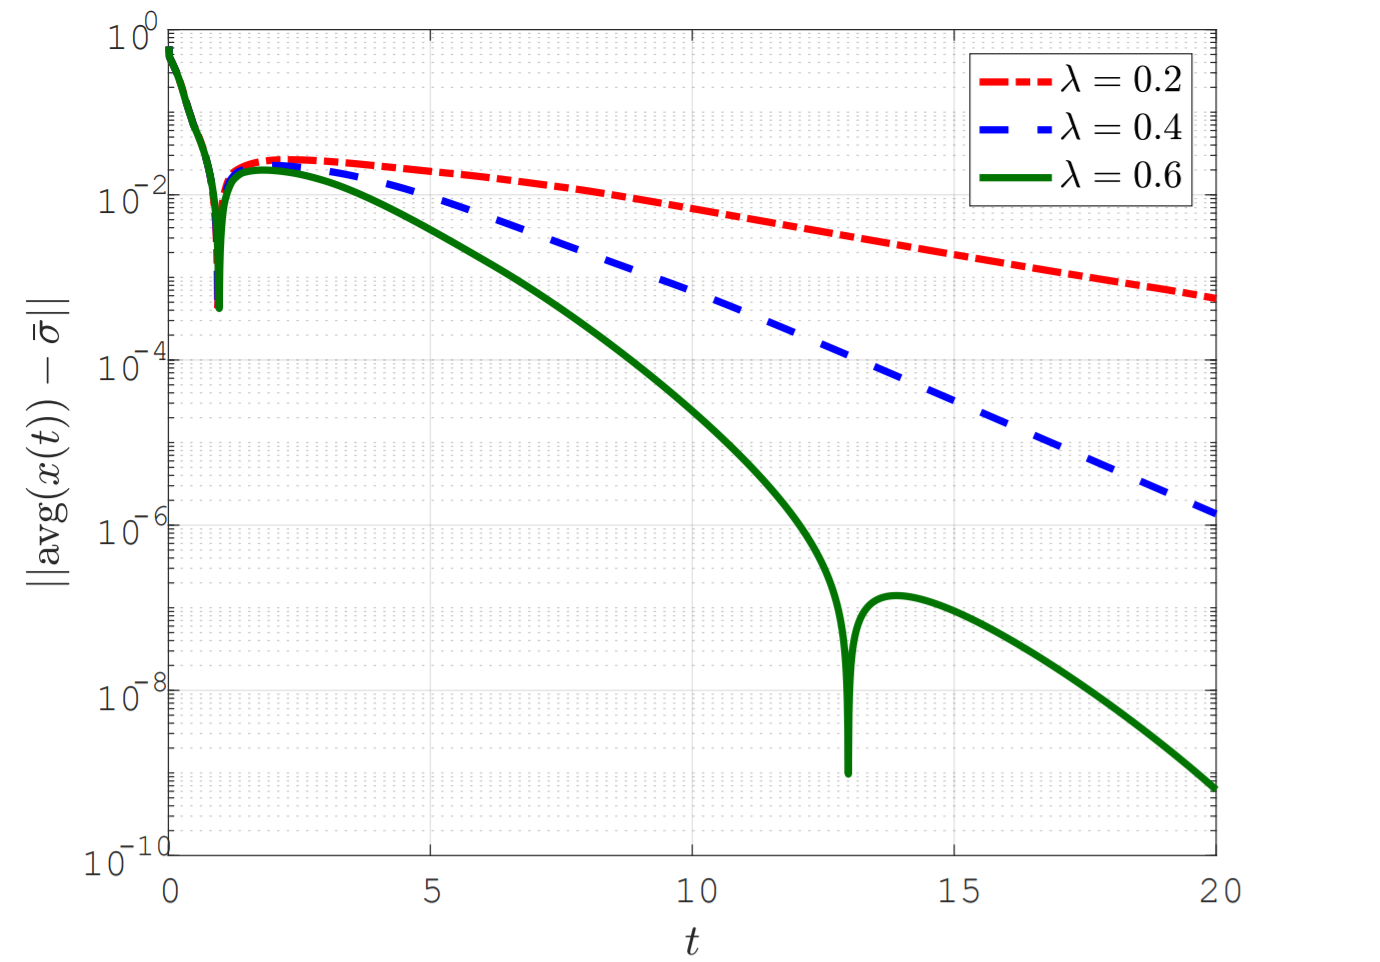
\includegraphics[width=8cm]{plot11.png}
		\caption{Відстань між середніми стратегіями досліду та рівноваги.}
		\label{secert_sharing_figures}
	\end{figure}

\end{columns}

\end{frame}

\begin{frame}{Алгоритм динаміки неперервного часу}{Числовий експеримент}
    	\begin{figure}
		\centering
		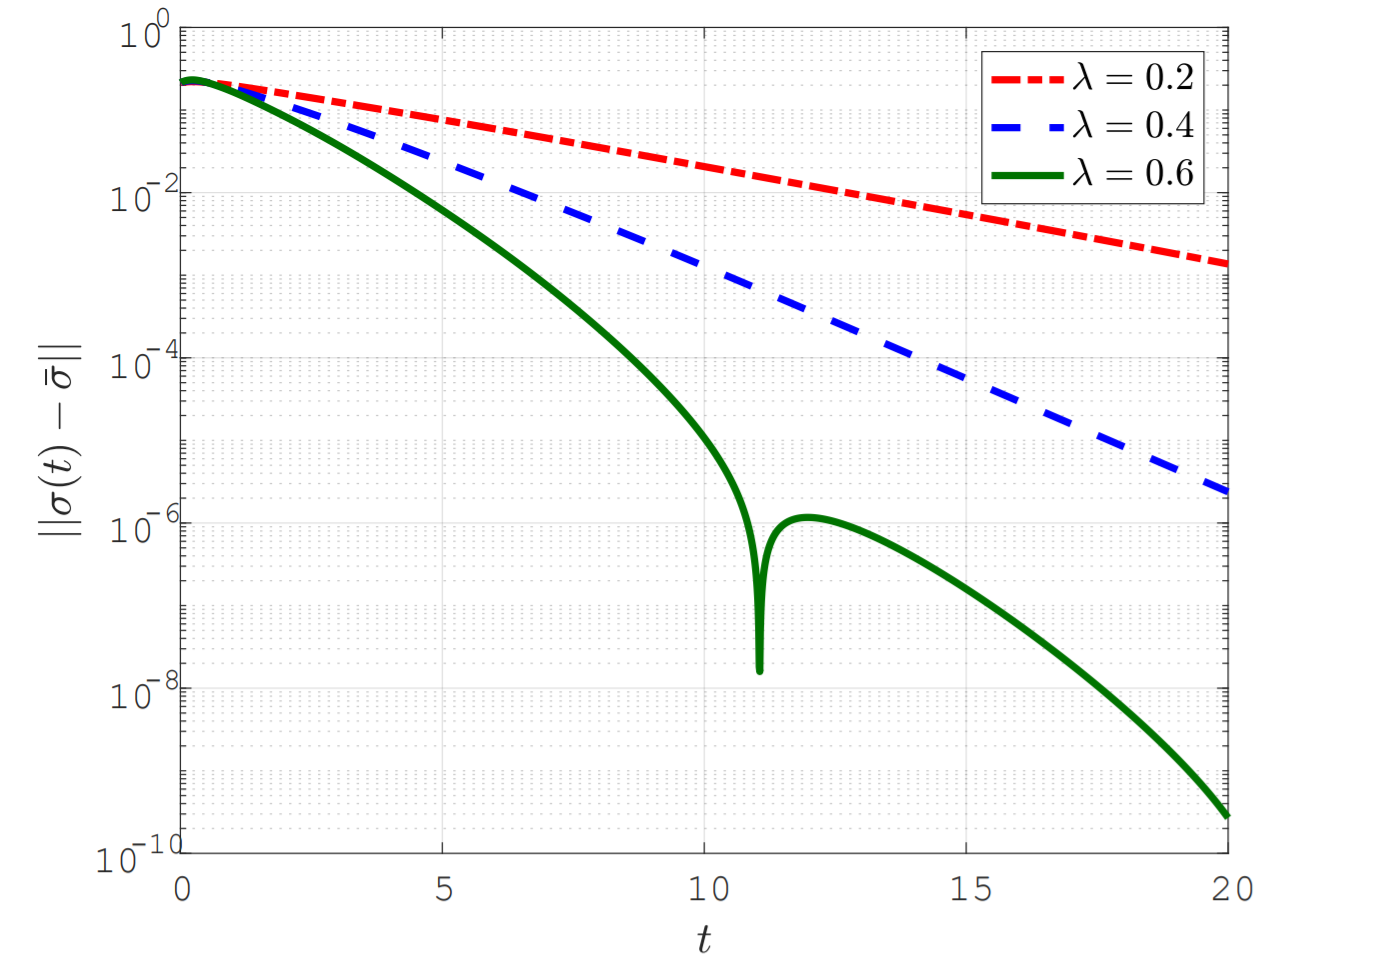
\includegraphics[width=9cm]{plot22.png}
		\caption{Відстань між інтегральним керуючим сигналом та його рівновагою.}
		\label{secert_sharing_figures}
	\end{figure}
\end{frame}

\begin{frame}{Лінійно збіжний алгоритм}{Постановка задачі}
    Розглянемо $n = 20$ фірм, що контролюють $L = 10$ локацій, кожній фірмі $i$ потрібно обрати її продукцію $g_{il}$, та знижки $s_{il}$ на локації $l$.

Ціну продукції фірми $i$ на локації $l$ позначимо як $c_{il}(g_{il})$ та визначимо як
$c_{il}(g_{il}) = a_{il}g_{il} + b_{il}g_{il}^2,$ де $a_{il}$ та $b_{il}$ параметри фірми $i$.

Дохід фірми $i$ на локації $l$ є $s_{il}p_{l}(s_l)$ де $s_l = \sum_{i=1}^{n} s_{il}$ загальна знижка локації та $p_{l}$ відповідна функція ціни.

Функція ціни $p_l$ є функцією резервного попиту та визначається як $p_l(s_l) = d_l - s_l,$ де $d_l$ це параметр локації $l$.

Місткість продукції фірми $i$ на локації $l$ запишемо як $cap_{il}$.

У симуляції було покладено $a_{il} \sim U(2,12), b_{il} \sim U(2,3), d_l \sim U(90,100)$ та $cap_{il} = 500$ для $i = 1, ..., n$ та $l = 1, ..., L.$ де $U(u_1,u_2)$ рівномірний розподіл на інтервалі $[u_1, u_2]$.

\end{frame}

\begin{frame}{Лінійно збіжний алгоритм}
Взаємодія гравців між собою описується матрицею ваг $W = \{w_{ij}\}_{n\times n}$ де $w_{ij} > 0$ якщо гравці спілкуються, та $w_{ij} = 0$ в іншому випадку.

Спочатку для кожного гравця $i \in N$ обираємо стратегію $\mathbf{x}_i^0 \in X_i$ випадковим чином та $\mathbf{v}_i^0=\mathbf{x}_i^0$.

Повторюємо наступну процедуру для всіх гравців $i \in N$ допоки не зійдемось. 
\begin{align}
\mathbf{\hat{v}}^{k+1}_i &= \sum_{j=1}^{n} w_{ij}\mathbf{v}^k_i,\\
\mathbf{\hat{x}}^{k+1}_i &= \mathbf{x_i^k-\alpha f_i\left(\mathbf{x_i^k},\mathbf{\hat{v}}^{k+1}_i\right)},\\
\mathbf{x}^{k+1}_i &= \mathbf{x}^{k}_i + \beta\left(\mathbf{\hat{x}}^{k+1}_i-\mathbf{x}^{k}_i\right),\\
\mathbf{v}^{k+1}_i &= \mathbf{\hat{v}}^{k+1}_i + \mathbf{x}^{k+1}_i-\mathbf{x}^{k}_i.
\end{align}
де $\alpha$ оберемо, щоб послідовність $\{\mathbf{x}^k\}_{k\in \mathbb{N}}$ збігалась до фіксованої точки $\mathbf{x}^*$, $\mathbf{v}_i$ вектор, що змінюється від дій сусідів, $\alpha > 0$ та $\beta \in (0,1]$.

\end{frame}

\begin{frame}{Лінійно збіжний алгоритм}{Числовий експеримент}
    \begin{columns}
	\column{0.4\textwidth}
	Алгоритм було розглянуто для трьох випадків:
\begin{itemize}
\item{ \textit{Linear}: mod$(i+11j,n)+1,$

$0 \leq j < n/11.$}
\item {\textit{Log}: mod$(i+2^j,n)+1,$

$0 \leq j < \mathrm{log}_{2}~n.$}
\item \textit{Complete}: $j,\; 0 \leq j < n$;
\end{itemize}
Матриця ваг $W = \{w_{ij}\}$ задається так
\begin{eqnarray*}
w_{ij} =
\begin{cases}
0, (i,j) \notin E \\
\delta, (i,j) \in E, i\neq j\\
1-\delta \cdot d(i), i = j
\end{cases}
\end{eqnarray*}

	\column{0.6\textwidth}
	\begin{figure}
		\centering
		% Requires \usepackage{graphicx}
		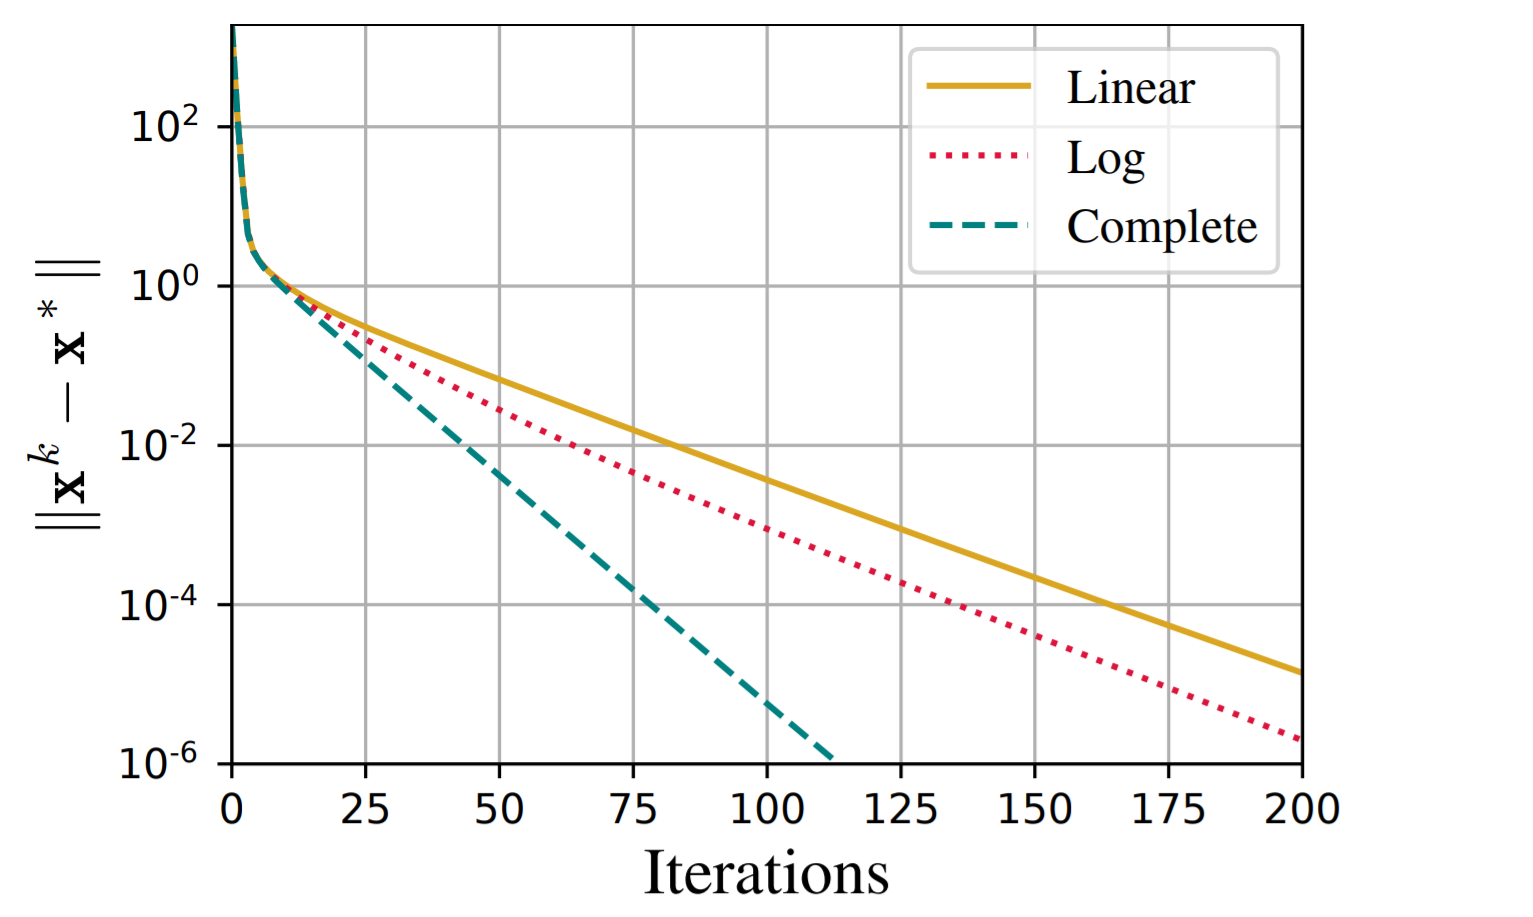
\includegraphics[width=8cm]{plot1.png}

	\end{figure}
	
\end{columns}
\end{frame}

\begin{frame}{Алгоритм розподіленого навчання}{Постановка задачі}
    У грі грають $N=10$ гравців. Граф зв’язку складається з неорієнтованого кола та 10 випадково вибраних ребер. Встановлюємо базову ціну $b_{0}=50$ та $b_{i}^{*} \sim U[3,7]$. Виробнича вартість $f_{i}$ містить кожну позицію $Q_{i}$, вибрану з $U[4.4,4.6]$, та кожну позицію $q_{i}$, вибрану з $U[1,1.2]$. Записи матриці суміжності $P^{*}$ рівномірно витягуються з $U[0.8,1]$ та пізніше упорядковуються, щоб мати одиничну суму по кожному рядку. Кожен запис невідомих ваг $H_{i}^{*}$ вибирається з $U[0.8,4.5]$. Гравець $i$ обирає кожен запис свого випадкового вектора дослідження з $U\left[-\delta_{i},+\delta_{i}\right]$, де $\delta_{i}=$ $\frac{0,01 }{2 \sqrt{n_{i}}} \min \left\{\mathcal{X}_{i j \max}: j=1, \ldots, n_{i}\right\}$.
\end{frame}

\begin{frame}{Алгоритм розподіленого навчання}{Алгоритм}
\noindent\textbf{Ініціалізація:} $\{y_{i}^{(0)}\},\{\hat{w}_{i}^{(0)}\}$ за допомогою $y_{ i}^{(0)} \in \mathcal{X}_{i}$ та $\hat{w}_{i}^{(0)} \in \mathcal{W}_{i}$\\
\textbf{Повторення поки не зійдеться:}\\
1) Оновлення кроку: запустити Підпрограму 1;\\
2) Оновлення оцінки параметра: запустити Підпрограму 2;\\
\textbf{Повертаємо:} $\{y_{i}^{(k)}\},\{\hat{w}_{i}^{(k)}\}$.\\
\end{frame}

\begin{frame}{Алгоритм розподiленого навчання}{Підпрограма 1}
\textbf{Доступні змінні:} $\{y_{i}^{(k)}\},\{\hat{w}_{i}^{(k)}\}$;\\
\textbf{На} $k$\textbf{-ій ітерації, кожен гравець} $i \in \mathcal{N}$ :

Отримує $\{y_{j}^{j(k)}\}_{j \in \mathcal{N}_{i}^{+}}$ та $\{y_{j}^{i(k)}\}_{j \in \mathcal{N}_{i}^{-}}$;

$
\begin{aligned}
\tilde{y}_{i}^{j(k+1)} &=y_{i}^{j(k)}-\tau_{i j} \rho(y_{i}^{j(k)}-y_{j}^{j(k)}), \quad \forall j \in \mathcal{N}_{i}^{+} ; \\
\tilde{y}_{i}^{i(k+1)} &=\underset{\tilde{y}_{i}^{i} \in \mathcal{X}_{i}}{\operatorname{argmin}}\{\mathbb{J}_{i}(\tilde{y}_{i}^{i} ; \tilde{y}_{i}^{+(k+1)}, \hat{w}_{i}^{(k)})+\rho\left(\sum_{j \in \mathcal{N}_{i}^{-}} y_{i}^{i(k)}-y_{j}^{i(k)}\right)^{T} \tilde{y}_{i}^{i}\\
&\hspace{7cm} +\frac{1}{2 \tau_{i 0}}\|\tilde{y}_{i}^{i}-y_{i}^{i(k)}\|_{2}^{2}\} \\
y_{i}^{(k+1)} &=y_{i}^{(k)}+\gamma^{(k)}(\tilde{y}_{i}^{(k+1)}-y_{i}^{(k)}) .
\end{aligned}
$\\
\end{frame}

\begin{frame}{Алгоритм розподiленого навчання}{Пiдпрограму 2}
\noindent\textbf{На} $k$\textbf{-ій ітерації:}\\
Кожен гравець $i \in \mathcal{N}$ :

Випадково вибирає коефіцієнт дослідження $\delta_{i}^{(k)}$;

Приймає рішення грати $\check{y}_{i}^{i(k+1)}:=y_{i}^{i(k+1)}+\delta_{i}^{(k)}-\bar{\delta}_{i} r_{i}^{-1}(y_{i}^{i(k+1)}-p_{i})$;

Спостерігає за $J_{i}(\check{y}_{i}^{i(k+1)} ; s_{i}^{(k)})$ та отримує $\{\breve{y}_{j}^{j(k+1)}\}_{j \in \mathcal{N}_{i}^{+}}$ від внутрішніх сусідів;

Оцінює невідомі параметри $\hat{w}_{i}^{(k+1)}$ розв'язуючи систему.

\begin{equation*}\label{prog2}
    \hat{w}_{i}^{(k+1)}:=\operatorname{argmin}_{w_{i} \in \mathcal{W}_{i}} \frac{1}{k+1} \sum_{t=0}^{k}\left(s_{i}^{(t)}-\left\langle\ell_{i}^{(t)}, w_{i}\right\rangle\right)^{2} .
\end{equation*}

\end{frame}

\begin{frame}{Алгоритм розподіленого навчання}{Числовий експеримент}
	\begin{figure}
		\centering
		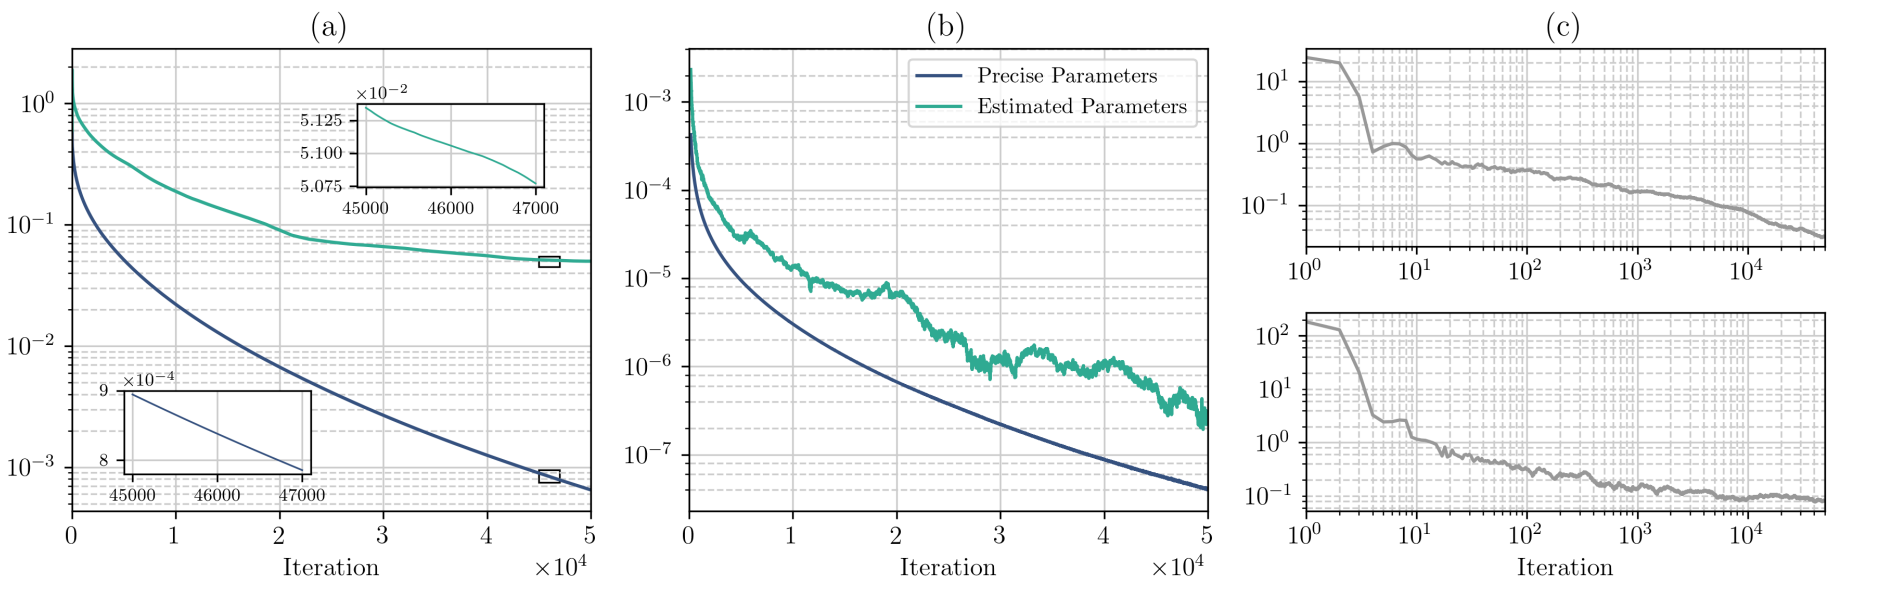
\includegraphics[width=12cm]{Fig_1.png}
	\end{figure}
	Продуктивність Алгоритму. (a) Нормовані відстані до справжньої рівноваги за Нешем. (b) Відносна довжина кроку оновлення на кожній ітерації. (c:1) Нормовані відстані оцінених ваг до точних ваг. (c:2) Нормовані відстані оцінених зміщень до точних зміщень.
\end{frame}

\begin{frame}{Алгоритм розподіленого навчання}{Постановка задачі}

У грі грають $N=10$ гравців. Гравці є виробниками деякої продукції, одиниця товару якою має певну початкову ціну $x_i$. Ціна формується з витрат виробника на одиницю товару та доходу, в задачі розглядаємо собівартість товару як 0, та максимальну ціну що може встановити виробник як 1.

Рівновагою Неша у даній грі є ситуація коли всі гравці продають товар по собівартості. Якщо припустити, що всі гравці продаватимуть товар по ненульовій ціні, то кожен гравець може змінити свою ціну на нижчу за мінімальну серед всіх гравців та переманити велику частку покупців.

Ціна за товар визначається випадково, як $x_i = 0.75 + 0.25 \cdot U(0,1)$.

Функція корисності гравців має вигляд $f_i(x_i,\overline{x}_i)=\frac{3}{4}\|x_i-x_i^*\|^2+(\overline{x}_i+0.5) \cdot x_i~,$

Матриця ваг $W = \{w_{ij}\}$ задається так
\begin{eqnarray}
w_{ij} =
\begin{cases}
\frac{1}{18}, & i\neq j\\
0.5, &  i = j
\end{cases}
\end{eqnarray}

\end{frame}

\begin{frame}{Frame Title}

\begin{figure}[h]
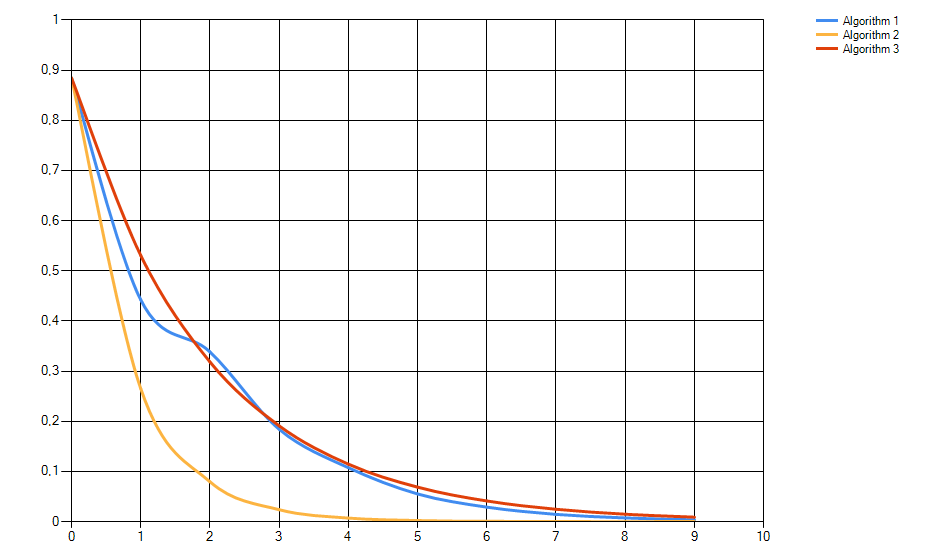
\includegraphics[scale=0.5]{Screenshot_1.png}
\caption{Середнє значення ціни між всіма гравцями впродовж часу.}
\end{figure}
\end{frame}

\begin{frame}{Висновки}
\begin{itemize}
    \item Розглянуто три алгоритми пошуку рівноваги Неша в мережево агрегативних іграх.
    \item Програмно реалізовано порівняння алгоритмів між собою.
    \item Чисельно проаналізовано збіжність всіх алгоритмів.
\end{itemize}
\end{frame}

\begin{frame}
    \begin{center}
        \huge{\textbf{Дякую за увагу!}}
    \end{center}
\end{frame}

\end{document}